 \documentclass[conference]{IEEEtran}
\IEEEoverridecommandlockouts
%\usepackage{hyphenat}
\usepackage[ruled,vlined]{algorithm2e}
\usepackage{amsmath}
\usepackage{xspace}
\usepackage[binary-units=true]{siunitx}
\usepackage{ulem}
%\usepackage{censor}
\usepackage[table]{xcolor}
\usepackage{graphicx}
\usepackage{hyperref}
\usepackage{tabularx}

\usepackage{subcaption}
\usepackage{booktabs}
\usepackage{multirow}
\usepackage{listings}
\usepackage{dingbat}
\usepackage{mathtools}

\hypersetup{
    colorlinks=true,
    linkcolor=black,
    citecolor=blue,
    filecolor=black,
    urlcolor=blue}

\def\BibTeX{{\rm B\kern-.05em{\sc i\kern-.025em b}\kern-.08em
    T\kern-.1667em\lower.7ex\hbox{E}\kern-.125emX}}


\makeatletter
  \def\footnoterule{\kern-3\p@
  \hrule \@width 2in \kern 2.6\p@} % the \hrule is .4pt high
\makeatother


\begin{document}

\newcommand{\fslspm}{FSL-SPM\xspace}
\newcommand{\fslafni}{FSL-AFNI\xspace}
\newcommand{\afnispm}{AFNI-SPM\xspace}
\newcommand{\tristan}[1]{\color{orange}\textbf{From Tristan:} #1\color{black}\xspace}
\newcommand{\ali}[2]{\color{green}\textbf{Ali:} #1\color{black}\xspace}



\title{Comparing tool variability and numerical variability in fMRI analyses}

\author{Ali Salari$^1$, Other Authors$^1$, Tristan Glatard$^1$ \\
$^1$ Department of Computer-Science and Software Engineering, Concordia University, Montreal, Canada}

\maketitle
\begin{abstract}

Numerical and software variability broadly affect structural, diffusion, and functional MRI analyses. Numerical
variability originates in software updates or code
parallelization, whereas software variability reflects discrepancies between
models implemented in different analysis software packages. While numerical
and software variability were both shown to impact analysis outcomes, the
extent to which these sources of variability compare for a given
analysis remains understudied. This work presents a comparison of
numerical and software variability for group-level and subject-level functional MRI analyses.
We reproduced a previous comparison between functional MRI analysis
software packages FSL, AFNI, and SPM, which we extended to measure
numerical variability through Monte-Carlo arithmetic.
Although We found that between-tool variability was larger than numerical variability,
we identified brain regions that numerical perturbations simulated between-tool variability.
Furthermore, we found more numerical instability in thresholded maps than unthresholded ones
and individual analysis than group-level analysis results.

\end{abstract}

\begin{IEEEkeywords}
  Numerical Instability, Reproducibility, Monte-Carlo arithmetic, Neuroimaging
\end{IEEEkeywords}


\section{Introduction}

% Data analysis workflows in many scientific domains have become increasingly complex and flexible.
Recent studies highlighted the instability of the neuroimaging pipelines depending on the computing platform,
software package, and even tool versions. Changes in the computational
environment such as compilers, libraries, operating systems may introduce small numerical errors and create
significantly different results in unstable pipelines~\cite{Glatard2015,Gronenschild2012,salari2020spot}.
Moreover, the impact of methodological changes on fMRI analyses has been investigated extensively~\cite{bowring2019exploring,botvinik2020variability,bhagwat2021understanding,carp2012plurality}.
For instance, in related works, it has been shown that running the same fMRI experiments by different teams can substantially affect
scientific conclusions~\cite{botvinik2020variability,carp2012plurality};
replication of fMRI experiments using the three most well-known software packages can influence the final determining areas of
brain activations~\cite{bowring2019exploring}; %bowring2021isolating.
also, the choice of preprocessing pipelines on neuroimaging cortical surface analyses is compound with instabilities~\cite{bhagwat2021understanding}.
% In the presence of such instabilities, it is often hard to trust the data processing results. % validity of the computational results.

In such a heterogeneous environment, numerical instability is an essential issue for reproducibility.
Numerical instability is a characteristic of pipelines that results from the influence of the floating-point arithmetics
and iterative convergence of numerical errors~\cite{freitas2002issue}.
Stochastic arithmetic approaches such as Monte-Carlo arithmetic (MCA)~\cite{Parker1997-qq} have been used to study the impact of numerical errors
originating in floating-point computations in mathematical libraries.
In~\cite{salari2021accurate}, we quantified the numerical stability of the HCP preprocessing pipeline~\cite{glasser2013} based on the MCA method
by creating a Fuzzy environment, so that instrument mathematical functions are implemented in mathematical system libraries.
As a result of numerical perturbations, we discovered a very low numerical precision in the result images comparable to the operating system variability.
In a related study~\cite{kiar2020numerical}, the instability of results was explored by instrumenting a connectome estimation pipeline with the MCA technique.
These works demonstrate the necessity of numerical uncertainty quantification for understanding related issues that hamper the computational reproducibility of analyses.

In this work, we reproduce an fMRI analysis in~\cite{bowring2019exploring} with different neuroimaging software packages in the presence of the Fuzzy environment,
and then quantify the variability across tools and the numerical variability in results.
We call the cross-software variation and numerical variation, between tool (BT) and within tool (WT) variability, respectively.
In fact, the WT variability shows results across software packages in the Fuzzy environment.
The primary objective of this study is to answer these two questions: 1) how the fMRI analyses across tools are numerically stable?
2) how the numerical variability is in comparison with the tool variability?
This comparative study reveals the importance of numerical variability and motivates research studies to evaluate the numerical uncertainty of the pipelines.

% We start to reproduce an analysis from Bowring, this can be as a practice for reproducibility manner in the community.
% In particular, we investigate the effect of 1) between software 2) within software (numerical)
% We present a comparative assessment of group-level analysis of an fMRI pipeline.


\section{Materials and Methods}

\subsection{fMRI analysis \& Dataset}

We replicated the fMRI analysis described as study `ds000001'
in~\cite{schonberg2012decreasing}, relying on the
data publicly available in OpenNeuro at
\url{https://openneuro.org/datasets/ds000001} and using the three main
software packages for fMRI data processing, namely FMRIB Software Library
(FSL)~\cite{jenkinson2012fsl}, Analysis of Functional NeuroImages
(AFNI)~\cite{cox1996afni}, and Statistical Parametric
Mapping(SPM)~\cite{penny2011statistical}. We selected this dataset because
comparable analysis pipelines implemented in FSL, AFNI and SPM 
were already published and extensively described in~\cite{bowring2019exploring}.
Furthermore, the work in~\cite{bowring2019exploring} already evaluated the effect of tool variability for
this dataset, which we intended to complement with the present quantification of numerical variability.

In the selected study, 16 healthy adult subjects participated in the
balloon analog risk task~\cite{lejuez2002evaluation} to measure
risk-taking behavior over three scanning sessions~\cite{schonberg2012decreasing}.
We reused the preprocessing, first-level, and
second-level analyses implemented by~\cite{bowring2019exploring} consistently across all three software packages using 
widely accepted analytical steps. Table~\ref{table:pipeline-steps} summarizes the analytical steps in each pipeline.
More details are available in~\cite{bowring2019exploring}.


%%%%%%%%%% Summary of statstics %%%%%%%%
\setlength{\tabcolsep}{4pt}
\begin{table}[h]
    \centering
    \begin{tabular}{|c|l|c|c|c|}
        \hline
%        \multirow{2}{*}{} & \multicolumn{1}{c}{Thresholded}& & \multicolumn{1}{c}{Unthresholded}& \\
        \multicolumn{2}{|c|}{} & FSL & AFNI & SPM \\
        \hline
        {Preprocessing} & {Motion Correction}                          & \checkmark    & \checkmark     & \checkmark  \\
        {} & {Segmentation}                               &    &      & \checkmark  \\
        {} & {Brain Extraction (Anatomical)}              & \checkmark     & \checkmark    & \checkmark  \\
        {} & {Brain Extraction (Functional)}              &   & \checkmark     &  \\
        {} & {Intra-subject Coregistration}               & \checkmark    & \checkmark     & \checkmark \\
        {} & {Inter-subject Registration}                 & \checkmark    & \checkmark     & \checkmark \\
        {} & {Analysis Voxel Size}                        & \checkmark    & \checkmark     & \checkmark \\
        {} & {Smoothing}                                  & \checkmark    & \checkmark     & \checkmark  \\
        \hline
        {First-level} & {Model Specification}                          & \checkmark    & \checkmark     & \checkmark  \\
        {} & {Inclusion of 6 Motion Parameters}                               & \checkmark   &  \checkmark    & \checkmark  \\
        {} & {Model Estimation}                           & &     & \checkmark  \\
        {} & {Contrasts}                                   &  \checkmark & \checkmark     & \checkmark \\
        \hline
        {Second-level} & {Model Specification}                          & \checkmark    & \checkmark     & \checkmark  \\
        {} & {Model Estimation}                           &      &    & \checkmark  \\
        {} & {Contrasts}                                   &   & \checkmark     & \checkmark  \\
        {} & {Second-level Inference}                               &  \checkmark  &    \checkmark  & \checkmark  \\
        \hline

      \end{tabular}
    \caption{Software processing steps (adapted from~\cite{bowring2019exploring}).}
    \label{table:pipeline-steps}
\end{table}

\subsection{Fuzzy libmath environment}

To introduce controlled amounts of numerical error in the analyses, we used the Fuzzy Libmath (FL) library~\cite{salari2021accurate}, an MCA-instrumented 
version of the GNU mathematical library (libmath).
FL works based on the MCA, a floating-point arithmetic that simulates roundoff and catastrophic cancellation errors
by introducing a controlled amount of noise in the floating-point operations 
through the following perturbation model~\cite{Parker1997-qq}:

\begin{equation} \label{eq:mca_inexact}
  inexact(x) = x + 2^{e_x-t}\xi
\end{equation}

where $e_x$ is the exponent in the floating-point representation of $x$,
$t$ is the virtual precision, the number of bits in mantissa that will not be perturbed,
and $\xi$ is a random uniform variable of $(-\frac{1}{2}, \frac{1}{2})$.
The MCA perturbations are automated using Verificarlo tool~\cite{denis2015verificarlo} at compilation time.

The instrumented functions are loaded in the pipeline using LD\_PRELOAD, a Linux environment variable
to force load a shared library into an executable. This allows functions defined in FL to transparently
overload the original ones without the need to modify or recompile the analysis pipeline.

FL only introduces perturbations in the output values of mathematical
functions but not in their implementation. This is done by wrapping the original functions 
and applying function \texttt{inexact} to their returned values.
Listing~\ref{algo:wrapper} shows an example of this wrapping for the log function in both single and double precisions.
In this script, the original functions are called by \texttt{dlsym},
a function that returns the memory address of a symbol, in our case \texttt{RTLD\_NEXT}, the address of the next occurrence of the function.
These wrappers are compiled with Verificarlo for each function. The MCA
instrumentation is activated by adding a floating-point zero to the output
of the original function so that this summation is instrumented.


% \lstdefinestyle{customc}{
%   belowcaptionskip=1\baselineskip,
%   breaklines=true,
%   frame=L,
%   xleftmargin=\parindent,
%   language=C,
%   showstringspaces=false,
%   basicstyle=\footnotesize\ttfamily,
%   keywordstyle=\bfseries\color{green!40!black},
%   commentstyle=\itshape\color{purple!40!black},
%   identifierstyle=\color{blue},
%   stringstyle=\color{orange},
% }

\lstdefinestyle{customasm}{
  belowcaptionskip=1\baselineskip,
  frame=L,
  xleftmargin=\parindent,
  language=[x86masm]Assembler,
  basicstyle=\footnotesize\ttfamily,
  commentstyle=\itshape\color{purple!40!black},
}
\lstinputlisting[caption=Sample wrapper script, label=algo:wrapper, style=customasm]{wrapper.c}
%\lstinputlisting[caption=Scheduler, style=customc]{../wrapper2.c}

FL allows measuring the effect of numerical variability by running a program multiple times, 
resulting in multiple independent realizations of the same analysis. Each of these samples 
are equally plausible estimates of the true numerical result. 
We used FL to simulate machine error, the relative error between a real number and its floating-point counterparts
(e.g., $2^{-53}$ for IEEE-754 double precision).
Moreover, FL allows simulating any virtual precision
by controlling the magnitude of the injected error and
thus to not be limited to the machine precision.

The presented method does not require any
particular software instrumentation in the data analysis code: it only
assumes that executables are dynamically linked against GNU libc. For this purpose,
(1) we captured the list of dynamic library dependencies using the \texttt{ldd} Linux utility for the software executables,
(2) we traced the system library calls using \texttt{ltrace} Linux program while running the pipeline processes.


\subsection{Data processing}

To measure between-tool (BT) variability, we executed the pipelines described in~\cite{bowring2019exploring}
with FSL version 5.0.10, AFNI version 18.1.09, and SPM12 version r7771
executed with GNU/Octave version 5.2.
All these software versions were identical to the original study except for SPM
that we used Octave instead of MATLAB to enable mathematical function instrumentation using FL,
while MATLAB uses its built-in functions and does not allow to apply FL.
We also used a fixed number of 7 threads in AFNI executions,
to reproduce similar results in~\cite{bowring2019exploring} in a feasible execution time.
All the analyses were conducted on the same operating system, CentOS 7.3.
We encapsulated the above-mentioned software packages in Docker container images with available Dockerfiles at \url{https://github.com/ali4006/fuzzy-neurotools/tree/main/dockerfile}.

The same subjects and analyses were conducted in the same configurations
with the FL environment, to measure within-tool (WT) variability. We
applied instrumentations at the virtual precision t=53 bits for
double-precision floating-point values and t=24 bits for single-precision
values. Three Fuzzy samples were generated for each subject and tool, to
match the number of tool samples.
We also captured further instrumentations for FSL tool for the virtual precisions ranged from 53 bits to 1 bit by steps of 2,
such that only double-precision was changed and single-precision was set to 24 bits for $t >= 24$ bits,
and both double- and single-precision simultaneously were changed for $t < 24$ bits.

We evaluated WT and BT variabilities in thresholded and unthresholded group-level and subject-level t-statistics maps.
We computed voxel-wise standard deviations of t-statistic values for each pair of tools
and then compared the standard deviations in both conditions.
We computed the WT standard deviation as the square root of the summation of variances between samples in each tool:

\begin{equation} \label{eq:mca_std}
  \begin{multlined}
  STD_{WT} = \sqrt{VAR_{tool1} + VAR_{tool2}}
%  VAR_{x} = \sum_{i=1}^{n} \frac{(x_i - \bar{x})}{n-1}
  \end{multlined}
\end{equation}

Moreover, we determined region-by-region Dice coefficients for the thresholded maps for each pair of tools.
We characterized 360 regions that correspond to the cortical parcellation atlas
in Human Connectome Project Multi-Modal Parcellation version 1.0 (HCP-MMP1.0)~\cite{glasser2016multi}.
Dice values in WT are computed as the average pair-wise Dices among three Fuzzy samples for each pair of tools.

\section{Results}
All scripts and data to create the figures presented in this section are available at \url{https://github.com/ali4006/fuzzy-neurotools} \tristan{move to lab org}.
The computations were performed on \href{https://www.computecanada.ca}{Compute Canada's} Béluga cluster
with 872 nodes, each with 2× Intel Gold 6148 Skylake @ 2.4 GHz (40 cores/node) CPU and node memory ranging from 92 to 752 GB.

We ensured a successful replication of the analyses initially presented in~\cite{bowring2019exploring}
by comparing t-statistic group maps with results in the original study.
We found identical checksums in the results of FSL.
Also, we could replicate results with the same SPM version and MATLAB as in the original study with visually imperceptible differences.
Changes in the SPM version and replacing Octave with MATLAB resulted in visually small differences which were still hard to distinguish between them.
For AFNI, the activation maps were similar overall; however, visual differences were noticeable.
This might be caused by the hardware optimizations such as dynamic scheduling~\cite{demmel2013numerical}.
We could confirm that AFNI results were passed the quality checks by visually assessing the registration results of each individual subject.

Summary statistics for the group-level unthresholded and thresholded t-statistics are reported in Table~\ref{table:pipeline-stats}.
Overall, BT variability was larger than WT variability for both means and standard deviations.
This was confirmed by computing the T-test and Wilcoxon signed-rank statistics between $BT(A, B)$, and $WT(A)$ and $WT(B)$ for $A$ and $B$ in $[FSL, SPM, AFNI]$.
We obtained statistically significant values between BT and WT variability with t-value $> 70$ and p-value $< 0.05$ in both thresholded and unthresholded maps.

%%%%%%%%%% Summary of statstics %%%%%%%%
\setlength{\tabcolsep}{5pt}
\begin{table}[h]
    \centering
    \begin{tabular}{cccc|cc}
        \toprule
        \multirow{2}{*}{}& {} & \multicolumn{2}{c}{Thresholded} & \multicolumn{2}{c}{Unthresholded} \\
        \cmidrule{3-4} \cmidrule{5-6} \\
        {} & {} & Mean & Std. dev. & Mean & Std. dev. \\
        \midrule
        \rowcolor{lightgray}
        {Between Tools} & FSL vs. SPM        &  1.282       & 0.525      & 0.443     & 0.344  \\
        \rowcolor{lightgray}
        {(BT)} & FSL vs. AFNI                &  1.548       & 0.616      & 0.547     & 0.441  \\
        \rowcolor{lightgray}
        {} & AFNI vs. SPM                    &  1.475       & 0.672      & 0.608     & 0.477  \\
        {Within Tool} & FSL                  &  0.354       & 0.491      & 0.082     & 0.065  \\
        {(WT)}   & SPM                       &  0.252       & 0.448      & 0.054     & 0.045  \\
        {}   & AFNI                          &  0.434       & 0.524      & 0.128     & 0.135  \\
        \bottomrule
    \end{tabular}
    \caption{Summary of voxel-wise mean and standard deviation in group-level t-statistics in BT and WT.}
    \label{table:pipeline-stats}
\end{table}


% \subsection{Comparing disparity in BT and WT}
%\subsection{Spatial localization of disparity in BT and WT}
\subsection{Group-level thresholded maps}

%Fig 1
Comparisons of standard deviations between thresholded images in WT and BT
on MNI space are shown in Figure~\ref{fig:thresh-maps}.
While we observed substantial BT variations with the average standard deviation 1.43,
the magnitude of WT variations was much smaller with the average standard deviation 0.34,
as was anticipated. 
Moreover, the magnitude of WT variations reached the magnitued of BT variations
in some regions, shown in white in Figure~\ref{fig:thresh-maps}-\textbf{C}.

% Fig2
Figure~\ref{fig:dice-thresh} compares regional normalized Dice coefficients of
activated voxels, showing a linear correlation between BT and WT with p-value $< 0.05$ in all three pairs.

%%%%%%%%%% Var. of Thresh %%%%%%%%
\begin{figure*}[ht]
    \fbox{\begin{minipage}{\dimexpr \textwidth-2\fboxsep-2\fboxrule}
      \centering
      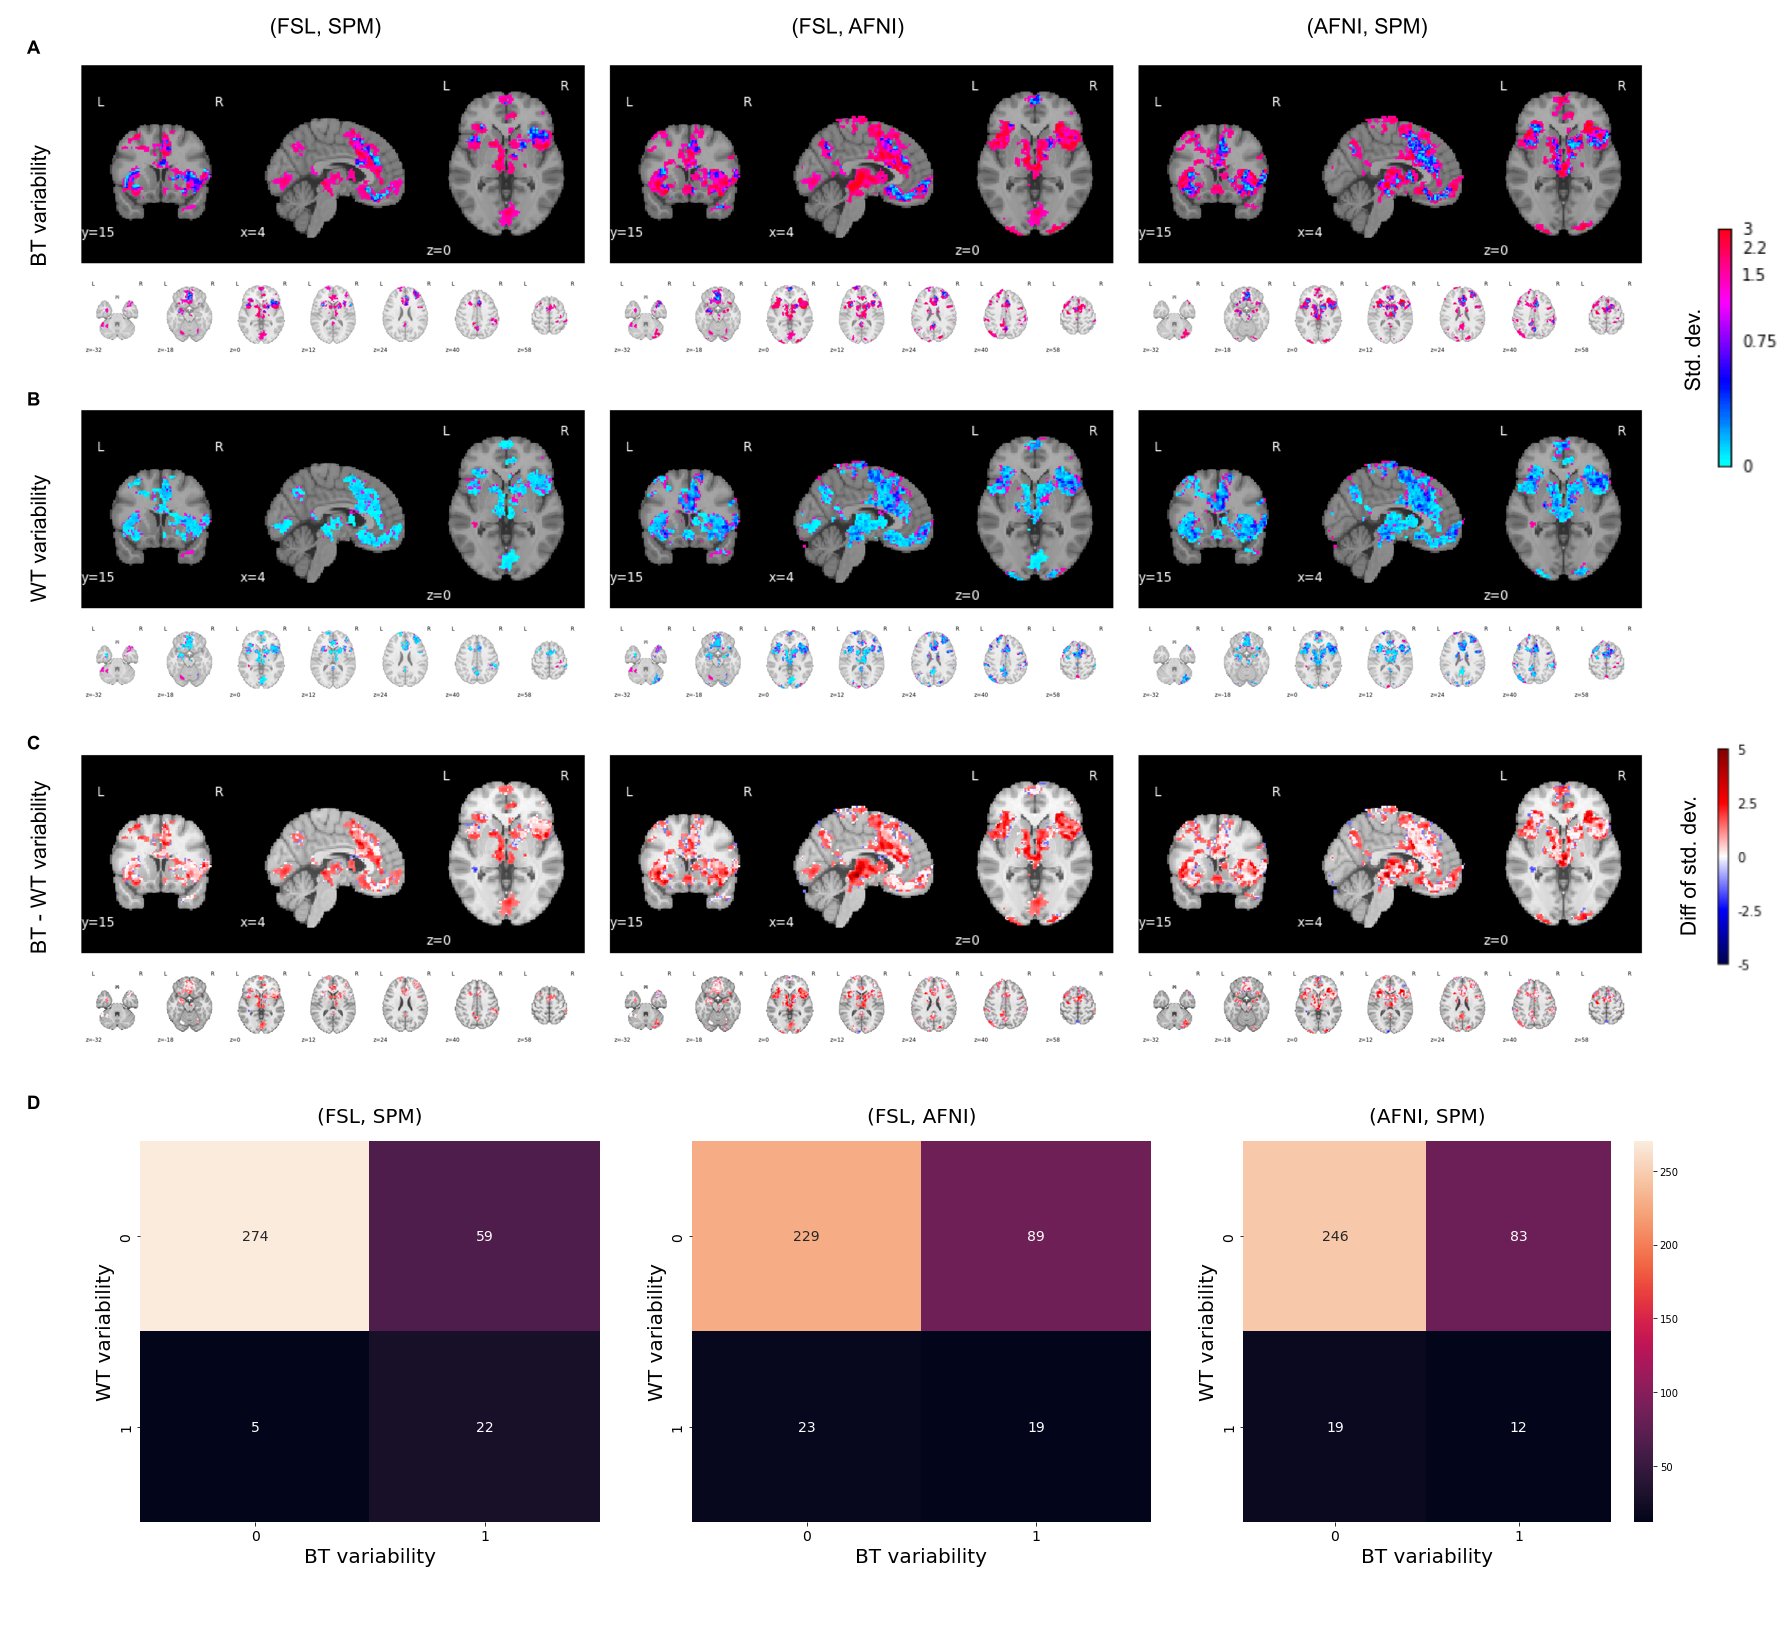
\includegraphics[width=\textwidth]{figures/std/gl-thresh.png}
      %\caption{Standard deviation of thresholded t-statistics map on template surface}
    \caption{Thresholded group t-statistics standard deviations computed between tools (\textbf{A}) and within tools (\textbf{B}), and difference between them (\textbf{C}). }
    % so that bright blue areas indicate more similar order of magnitude of variations in both conditions,
    %and vise versa for the darkder regions.}
    \label{fig:thresh-maps}
    \end{minipage}}
  \end{figure*}


  %%%%%%%%%% Dice plot of thresholded tstats%%%%%%%%
  \begin{figure}[ht]
    \fbox{\begin{minipage}{\dimexpr \columnwidth-2\fboxsep-2\fboxrule}
    \centering
    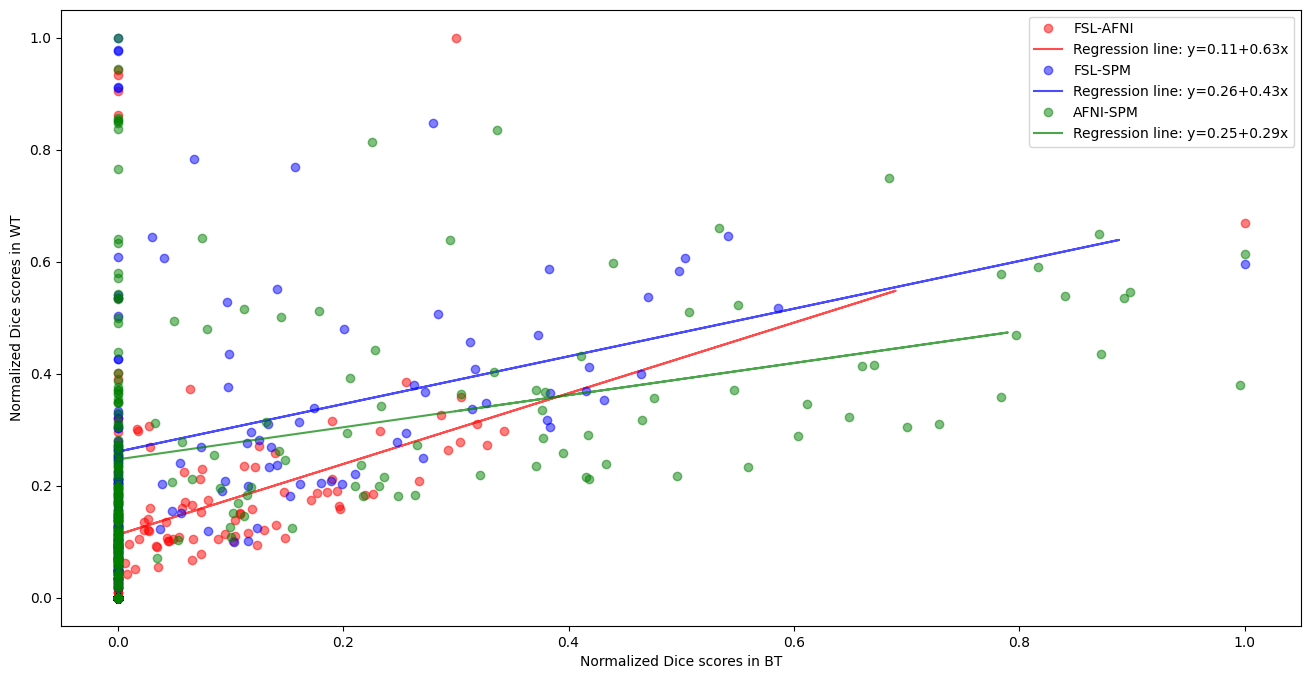
\includegraphics[width=\columnwidth]{figures/dices_corr.png}
    \caption{Normalized, regional Dice coefficients of activated voxels for
    BT and WT using the HCP-MMP1.0 parcellation of
    ~\cite{glasser2016multi}.}
    \label{fig:dice-thresh}
    \end{minipage}}
  \end{figure}



\subsection{Group-level unthresholded maps}
% \subsection{Variability of unthresholded statistical maps}

% Fig3
Similar conclusions are drawn from the unthresholded t-statistics maps
(Figure~\ref{fig:unthresh-maps}). BT variability is larger than WT variability overall, however,
BT and WT variability are comparable in some regions. 


%%%%%%%%%% Var. of Unthresh %%%%%%%%
\begin{figure*}[ht]
    \fbox{\begin{minipage}{\dimexpr \textwidth-2\fboxsep-2\fboxrule}
      \centering
      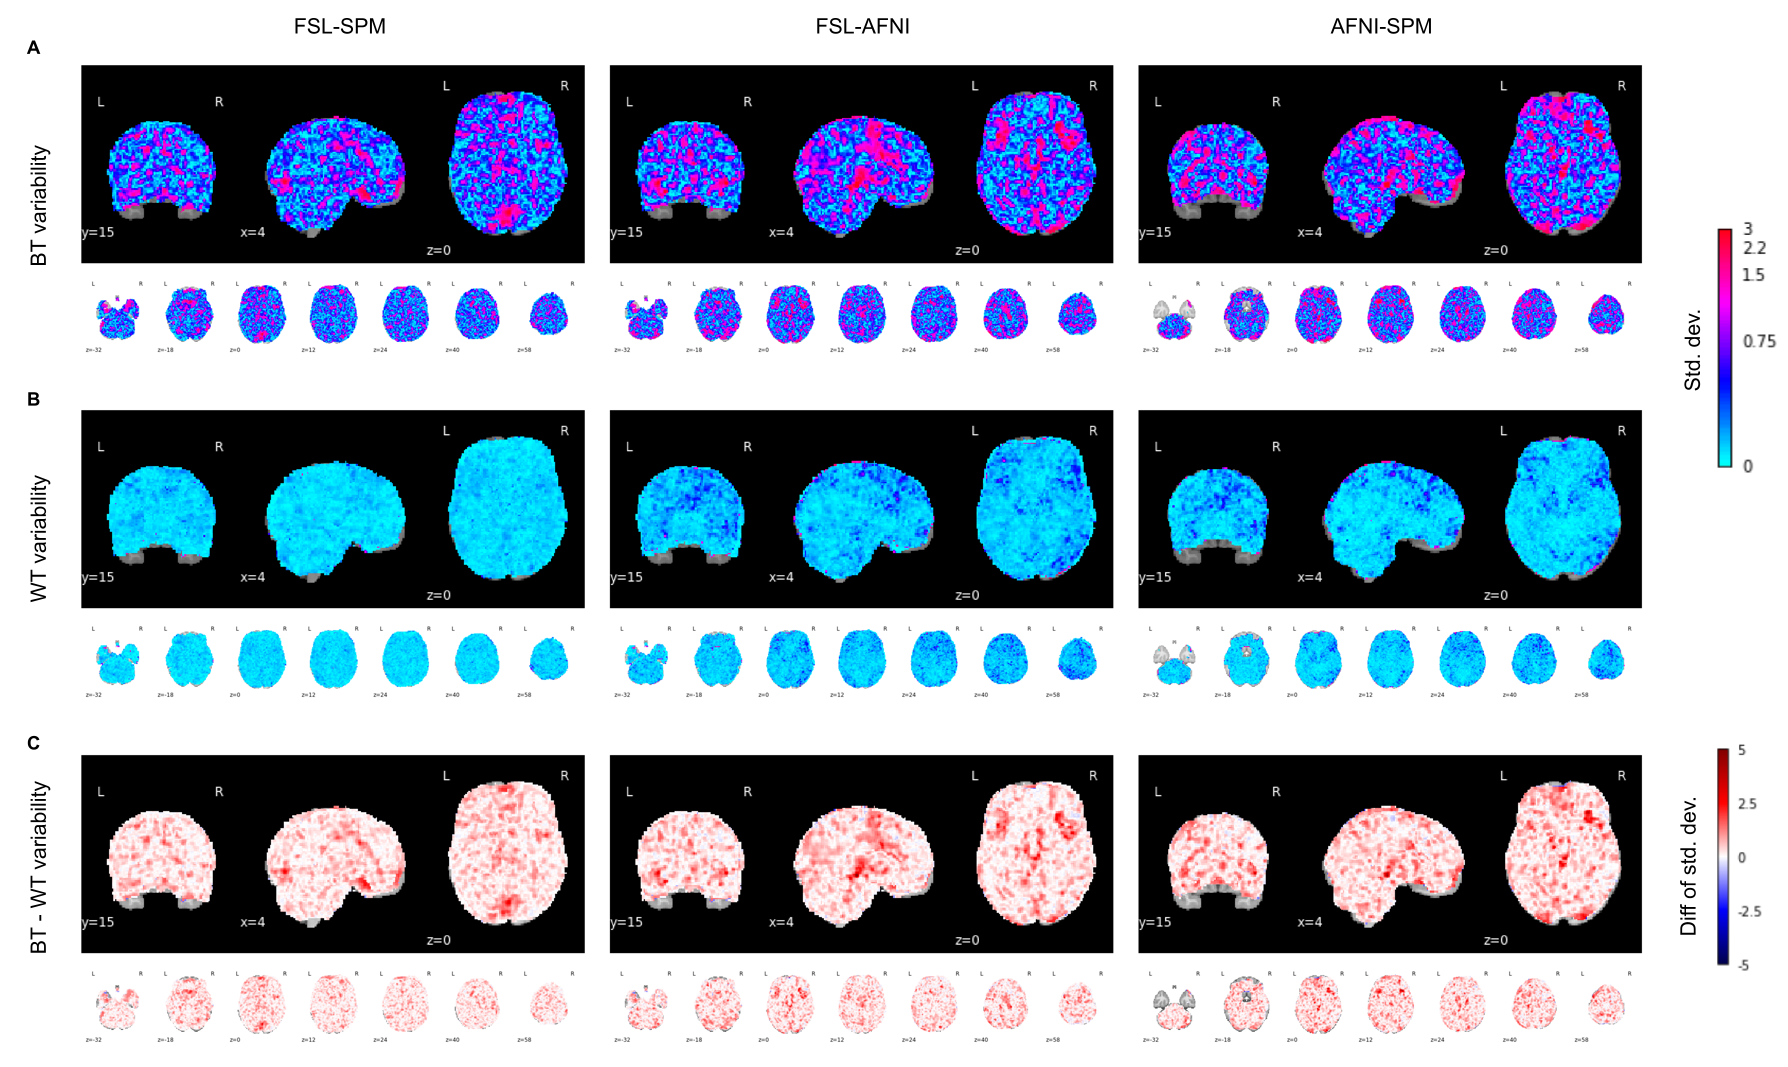
\includegraphics[width=\textwidth]{figures/std/gl-unthresh.png}
      %\caption{Standard deviation of thresholded t-statistics map on template surface}
    \caption{Unthresholded group t-statistics standard deviations computed between tools (\textbf{A}) and within tools (\textbf{B}), and difference between them (\textbf{C}).}
    \label{fig:unthresh-maps}
    \end{minipage}}
  \end{figure*}


% Fig4
Figure~\ref{fig:unthresh-correlation} highlights the voxel-wise standard deviations in WT and BT variability
with the identity lines that indicate voxels with the standard deviation of $BT = WT$.
The identity area is represented on MNI space in the second row in Figure~\ref{fig:unthresh-correlation}
for the voxels with the magnitude of standard deviation $> 0.1$ and the satndard deviation ratio of $0.5 < BT/WT < 2$.
The maps show the spatial localization of parts of the brain where the numerical variability simulated BT variability.
This refines the presented results in Figure~\ref{fig:unthresh-maps}-\textbf{C},
indicated voxels with similar magnitude of BT and WT variations were uniformly distributed across the brain.

  %%%%%%%%%% Corr. plot of tstats%%%%%%%%
  \begin{figure*}[ht]
    \fbox{\begin{minipage}{\dimexpr \textwidth-2\fboxsep-2\fboxrule}
      \begin{subfigure}[ht]{\textwidth}
        \centering
        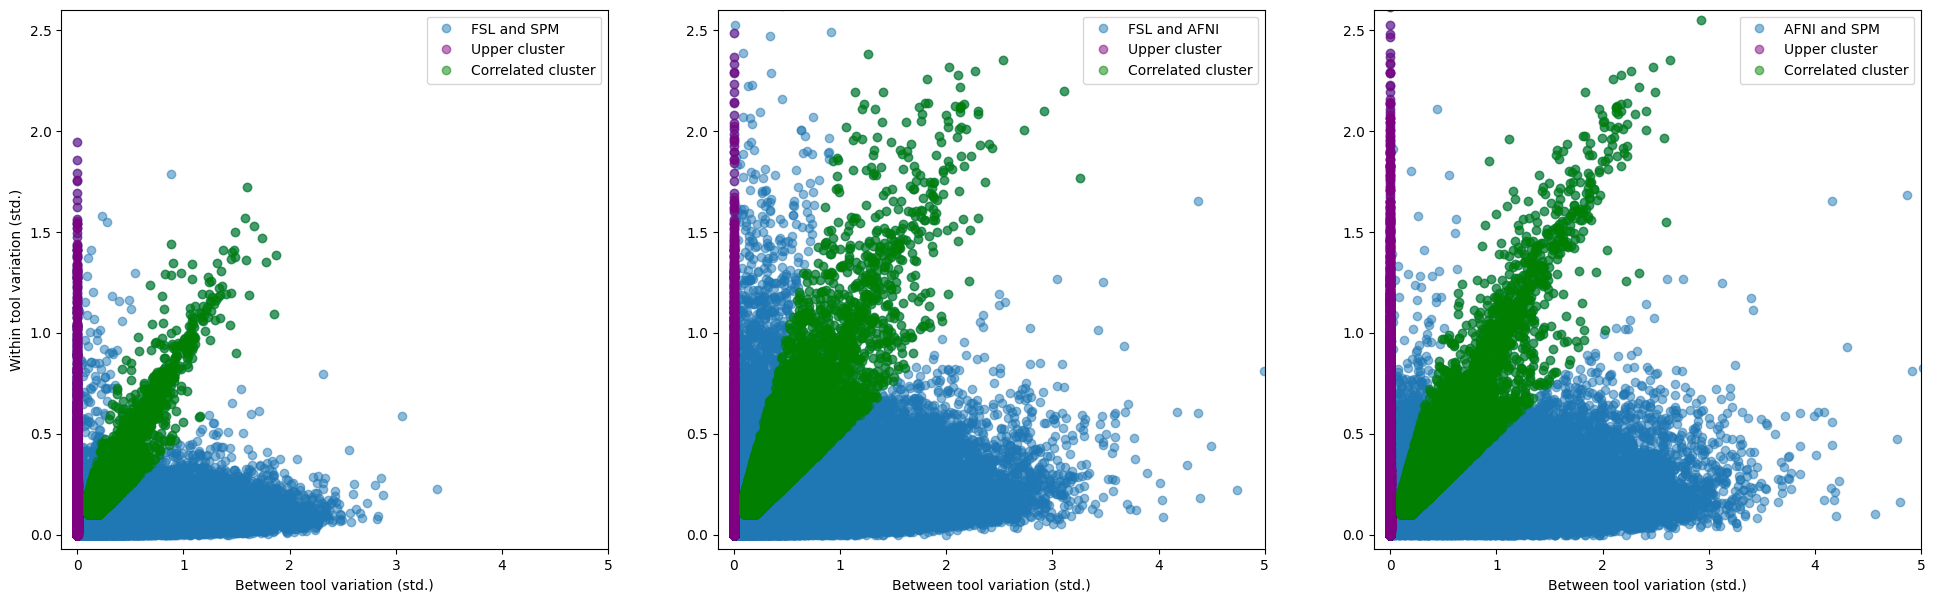
\includegraphics[width=\textwidth]{figures/std-corr-unthresh-plot.png}
        %\caption{Standard deviation of thresholded t-statistics map on template surface}
      \end{subfigure}
      \hfill
      \begin{subfigure}[ht]{\textwidth}
        \centering
        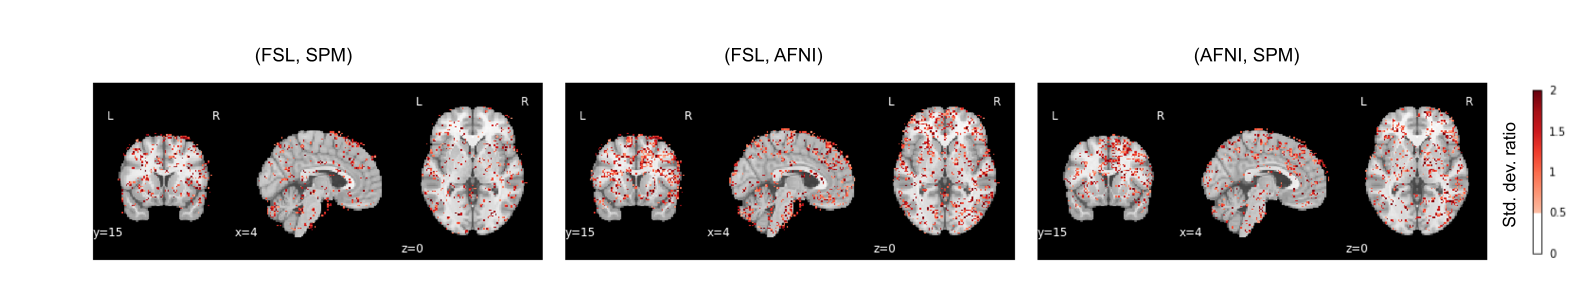
\includegraphics[width=\textwidth]{figures/std/correlated-unthresh.png}
        %\caption{Standard deviation of thresholded t-statistics map on template surface}
      \end{subfigure}
      \caption{
        Scatter plots of unthresholded group t-statistics standard deviations computed between tools and within tools.
        The identity line distinguishes voxels where the standard deviation BT is equal to WT.
        Voxels with the standard deviation ratio of BT/WT in the interval (0.5, 2) are represented on brain maps in the second row.}
    \label{fig:unthresh-correlation}
    \end{minipage}}
  \end{figure*}


  \subsection{Subject-level unthresholded maps}

  Figure~\ref{fig:unthresh-maps-sbj} shows BT and WT variability of the
  unthresholded t-statistics for the subject with the highest WT
  variability among the 16 subjects.
  We observed substantial WT variations with the average standard deviation 0.099 compared to 
  the average standard deviation 0.466 for BT variations.
  As can be seen in the Figure, WT variability approaches and even surpasses BT variability in some regions.
  This subject also revealed that WT variability mainly concentrated in some regions  
  contrary to the corresponding variability from unthresholded group-level t-statistics which was uniformly distributed across the brain.

  %%%%%%%%%% Var. of Unthresh sbj05%%%%%%%%
\begin{figure*}[ht]
  \fbox{\begin{minipage}{\dimexpr \textwidth-2\fboxsep-2\fboxrule}
    \centering
    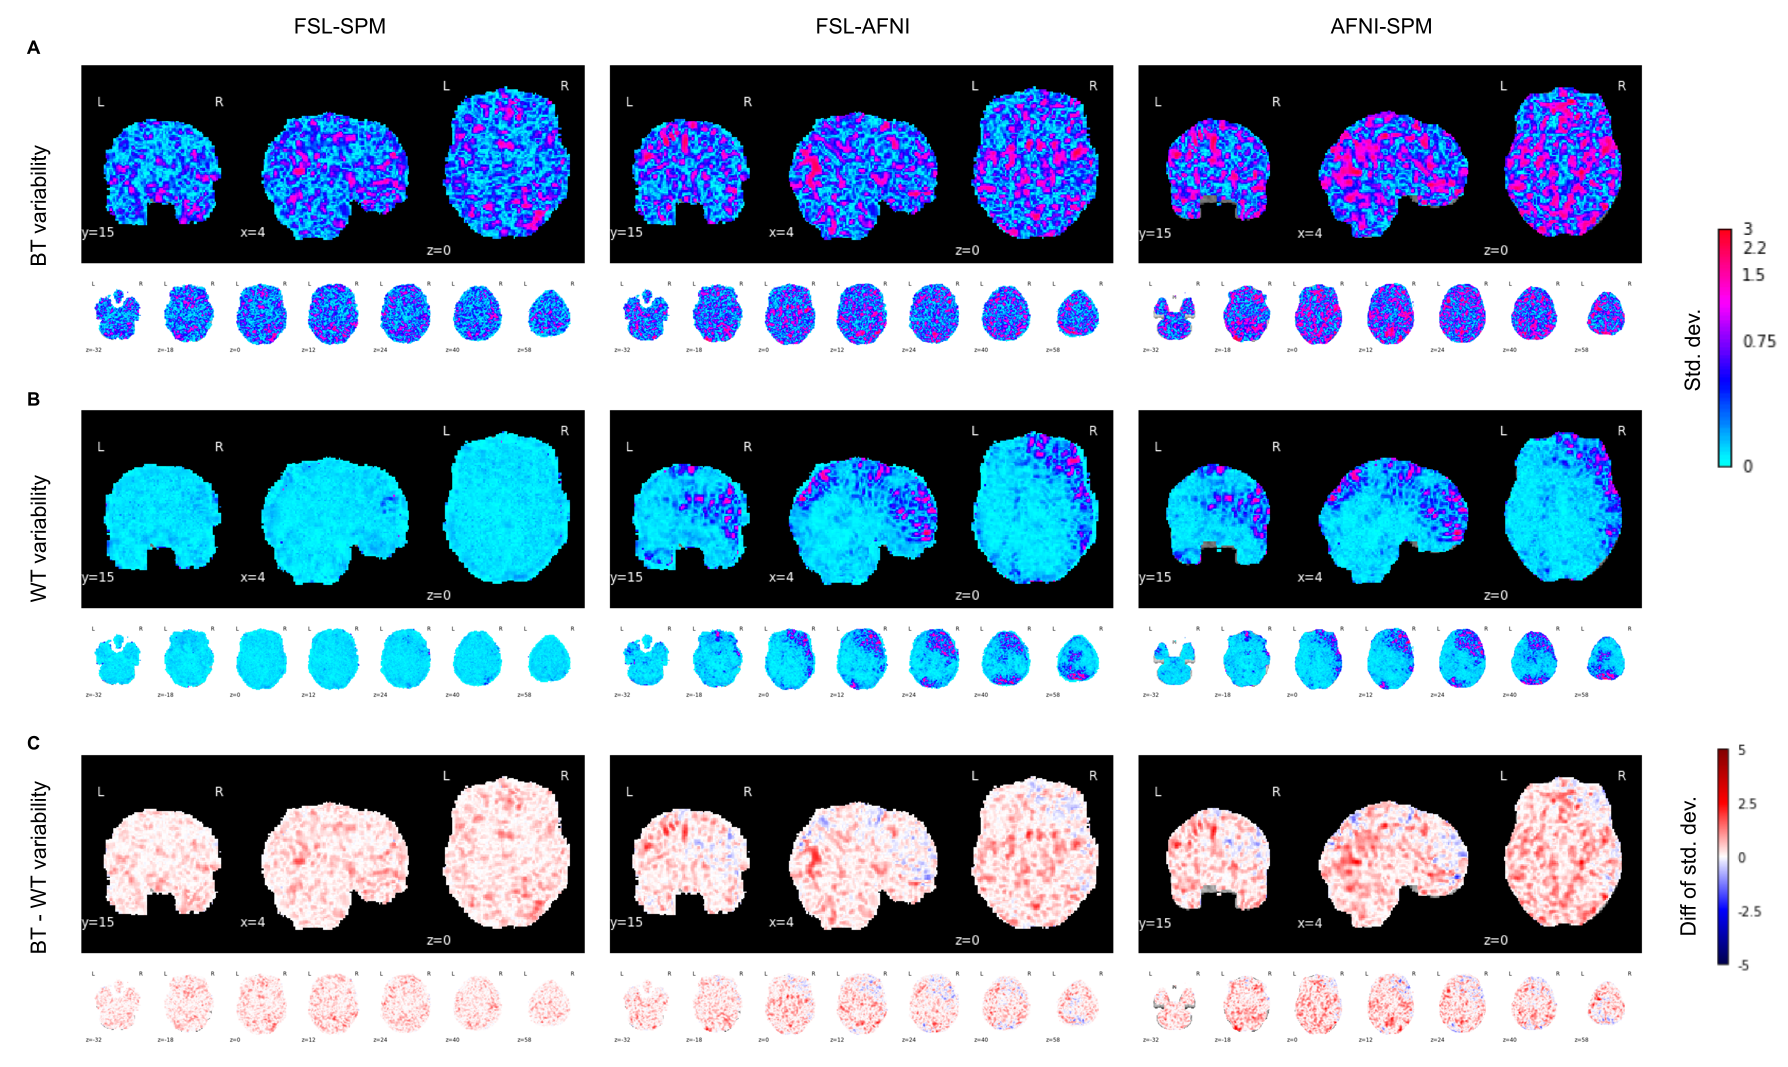
\includegraphics[width=\textwidth]{figures/std/sbj05-std.png}
    %\caption{Standard deviation of thresholded t-statistics map on template surface}
    \caption{Unthresholded subject t-statistics standard deviations computed between tools (\textbf{A}) and within tools (\textbf{B}), and difference between them (\textbf{C}).
    This is for the subject with the highest WT variability.}
  \label{fig:unthresh-maps-sbj}
  \end{minipage}}
\end{figure*}

\subsection{WT variability across virtual precisions}

While the previous results were obtained at the virtual precision of 53~bits for double-precision floating-point values
and 24~bits for single-precision values, we evaluated WT variability across different virtual precisions for FSL.
Figure~\ref{fig:across-precisions} represents the root-mean-square error (RMSE) between the standard deviations per voxel
in BT and WT resulted from the Fuzzy FSL,
substantiating that how variabilities in both conditions are close to each other across different virtual precisions.

We determined the virtual precision of t=17 bits as the precision that minimized the RMSE between BT and WT on average.
This is the precision that numerical perturbations in FSL more closely simulated BT variability.
The brain maps of standard deviations between BT and WT obtained from the Fuzzy FSL at t=17 bits (Figure~\ref{fig:gnp-mni})
show significant WT variability, particularly for some regions in the frontal, parietal, and limbic lobes, close to BT variability.


  %%%%%%%%%% plot different precisions%%%%%%%%
  \begin{figure}[ht]
    \fbox{\begin{minipage}{\dimexpr \columnwidth-2\fboxsep-2\fboxrule}
        \centering
        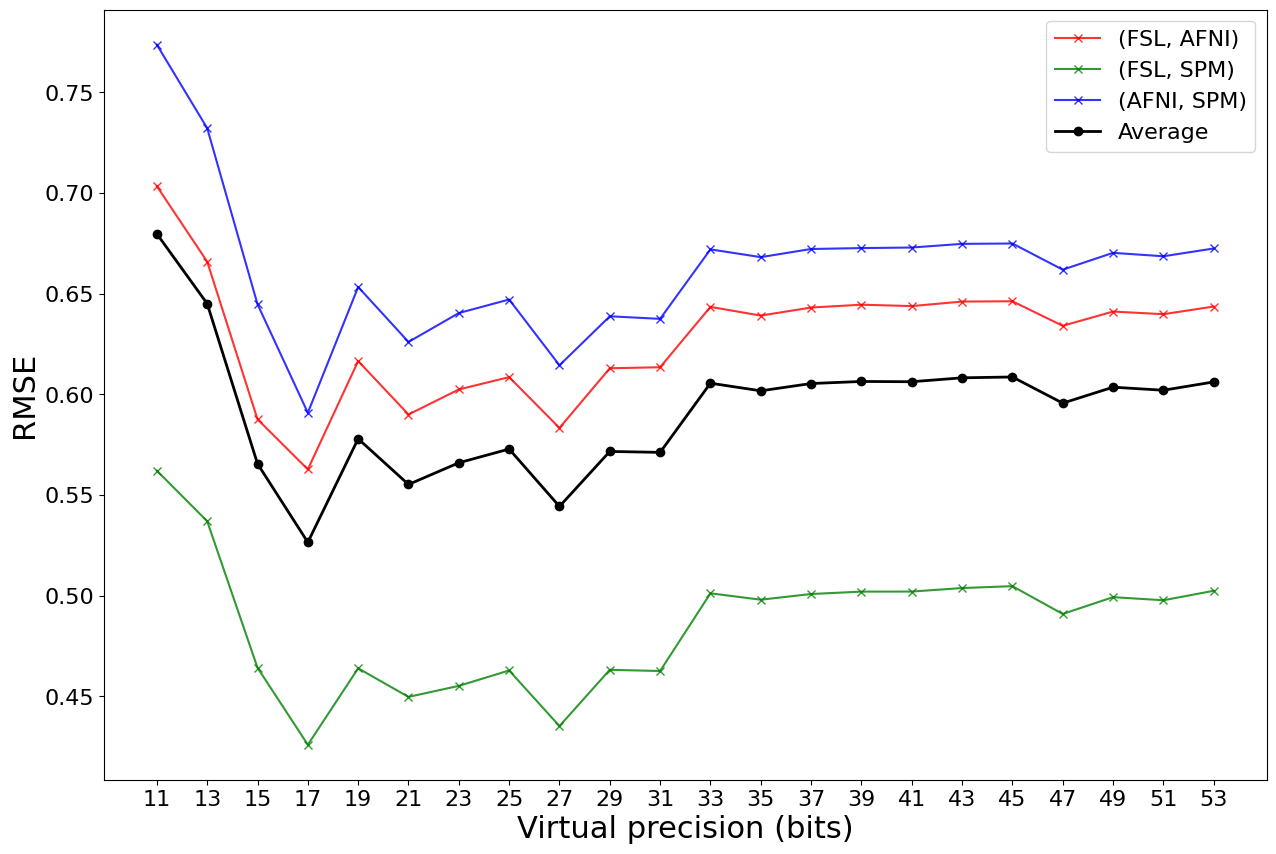
\includegraphics[width=\columnwidth]{figures/rmse-precisions.png}
        %\caption{Standard deviation of thresholded t-statistics map on template surface}
      \caption{Voxel-wise RMSE between BT and WT variability maps for different virtual precisions. WT is computed from three samples of FSL tool.}
    \label{fig:across-precisions}
    \end{minipage}}
  \end{figure}

  
  %%%%%%%%%% plot different precisions%%%%%%%%
  \begin{figure}[ht]
    \fbox{\begin{minipage}{\dimexpr \textwidth-2\fboxsep-2\fboxrule}
        \centering
        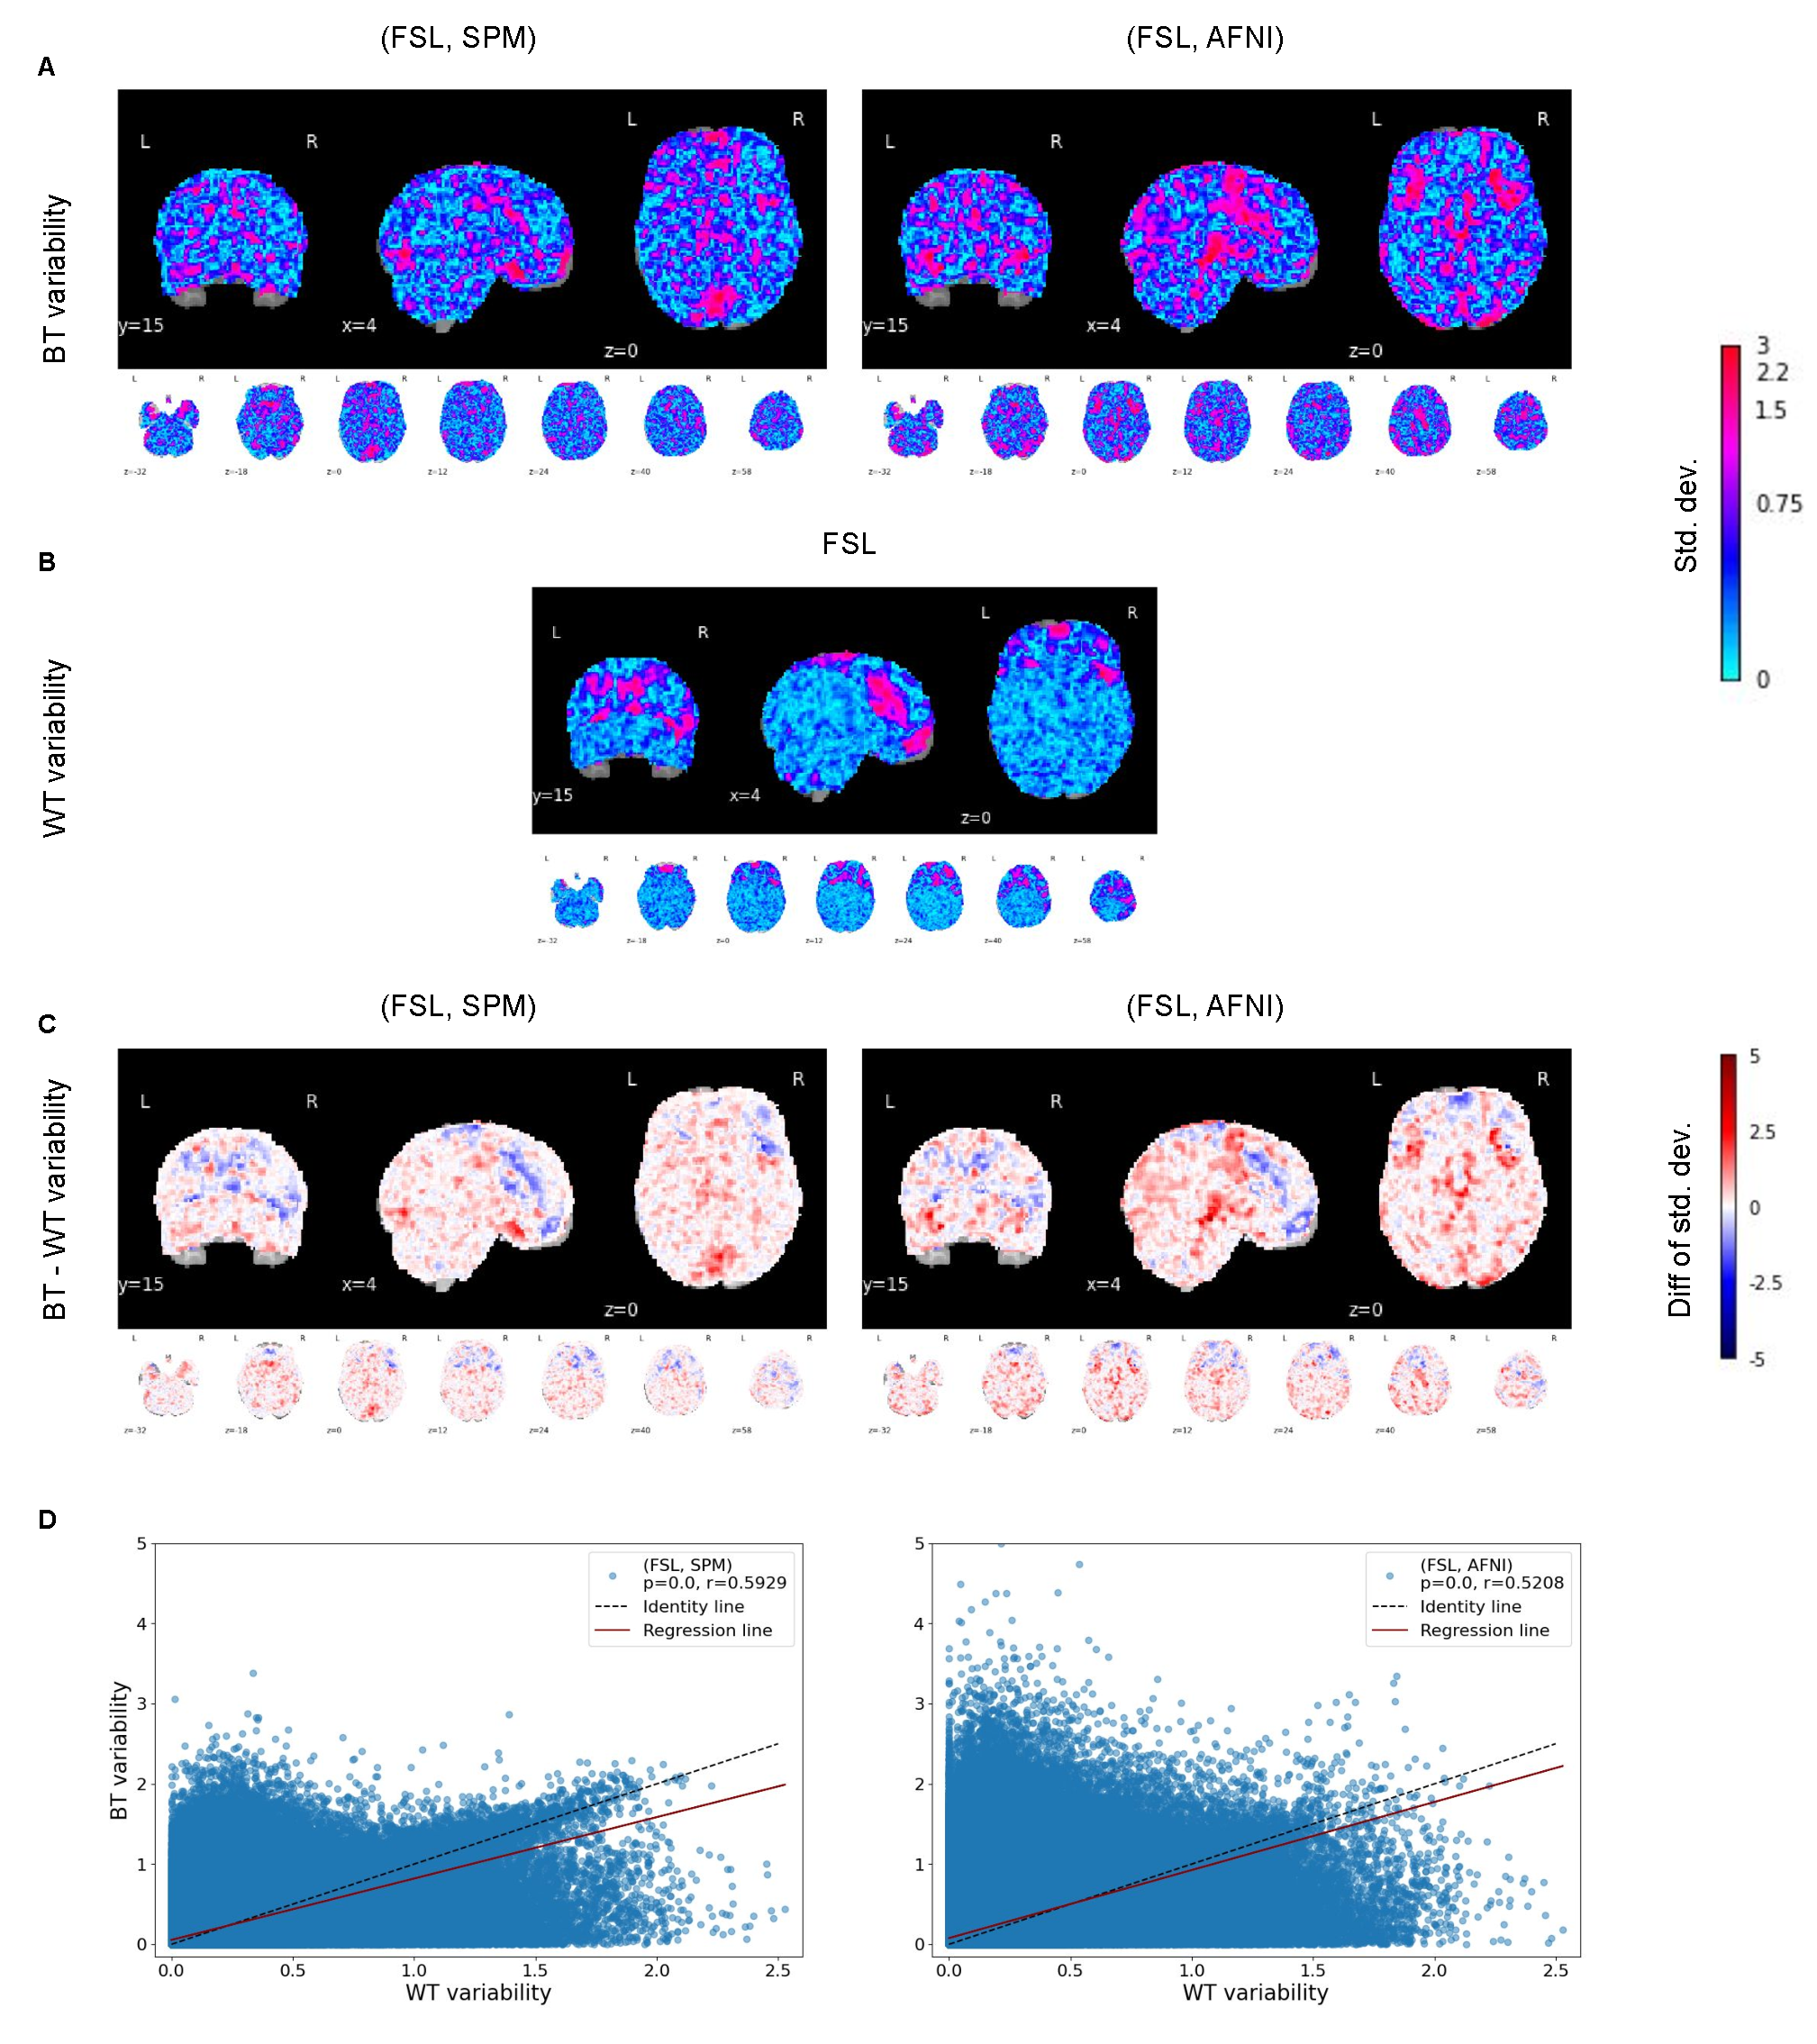
\includegraphics[width=\textwidth]{figures/bg_global_precision.pdf}
        %\caption{Standard deviation of thresholded t-statistics map on template surface}
        \caption{Unthresholded group t-statistics standard deviations computed between tools (\textbf{A}) and within tools (\textbf{B}), and difference between them (\textbf{C}).
        WT is computed from three samples of FSL tool at the virtual precision of t=17 bits.}
    \label{fig:gnp-mni}
    \end{minipage}}
  \end{figure}



\section{Discussion}

We represented differences in the results of an fMRI analysis between numerical variability
and the variability arisen from software package variations.
Although BT variability was larger than WT variability on average,
we demonstrated regions in the brain maps that numerical perturbations could simulate BT variability.
The correlation of these variabilities suggests that numerical perturbations can be used to evaluate the robustness of the analyses
to inter-software disparities.

While switching between \fslspm was generated the least BT and WT variabilities consistently, the most level of these variabilities was identified
between \fslafni and \afnispm. %We also found AFNI as the most sensitive tool to numerical perturbations.
These results do not indicate which software package is better or worse since there is no ground-truth model for the analyses.
However, this study revealed the importance of numerical instability in the selected tools for doing fMRI analyses.
It provided a view of related numerical variability of which should be taken into consideration by the software developers.

We found that numerical instability in individual analyses was attenuated in group analyses
since we obtained substantially higher variability in t-statistics at the level of subjects.
This is consistent with the findings in~\cite{bowring2021isolating} in which identified the first-level signal model as the largest
source of variability across the three tools for this study.
This is an issue for the development of fMRI biomarkers.
As a solution, we can aggregate the results obtained from numerical perturbations to improve biomarkers,
as suggested in~\cite{kiar2020numerical} where data augmentation using numerical perturbations resulted in a better classification in connectomics.

It is notable that we obtained more uncertainty on thresholded results than unthresholded maps, %This issue is 
probably due to different thresholding values used in different tools.
This is consistent with the observations in~\cite{bowring2021isolating} where identified a high correlation between unthresholded t-statistic maps,
but substantially low Dice coefficient for activations in the thresholded maps.
This raises further investigations on thresholding techniques to reduce instabilities.

Given that FL only perturbs basic mathematical functions, we expect more numerical variability by perturbing linear algebra,
in particular for non-scalar types like vectors or matrices. For the future study, this can be evaluated using MCA-instrumented versions 
of BLAS and LABACK along with other libraries available in the Fuzzy project in Verificarlo's GitHub repository at github.com/verificarlo/fuzzy.  


\section{Conclusion}

\begin{itemize}

    \item[$\bullet$ ] Further studies can be evaluating the numerical stabilities within tool by focusing on the particular parts of
    the pipeline that has been identified as the main sources of variations in~\cite{bowring2021isolating}.
    Also, we can invetigate the precision in WT variability that simulates mostly BT variability in the furure study.

\end{itemize}


\section{Acknowledgments}


%%
%% The next two lines define the bibliography style to be used, and
%% the bibliography file.
\bibliographystyle{plain}
\bibliography{biblio}


\end{document}
\endinput
%%
%% End of file `sample-authordraft.tex'.
